\section{Elektrostatische Analyse}
\subsection{Integralgleichungen}
\subsubsection{Gausssches Gesetz}
\begin{minipage}[c]{0.31\columnwidth}
    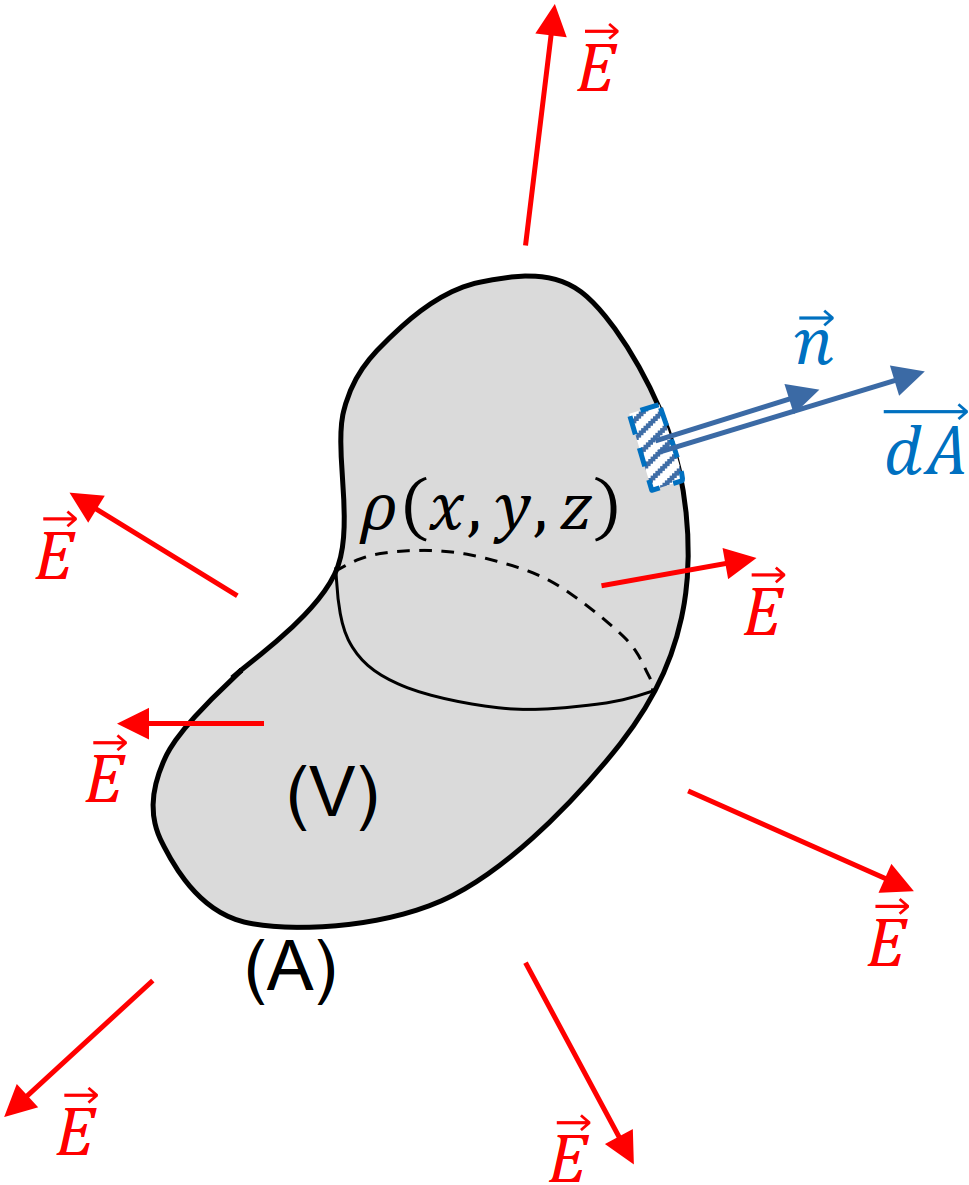
\includegraphics[width=\columnwidth]{images/V1B0.png}
\end{minipage}
\hfill
\begin{minipage}[c]{0.65\columnwidth}

Der Fluss des Vektors $\vec{D} = \varepsilon \cdot \vec{E}$ durch eine geschlossene orientierte Fläche ($A$) ist gleich der elektischen Ladung $Q$, die von der Fläche ($A$) umgeben ist:

    \[
        \boxed{\underset{(A)}{\operatorname*{\oiint}}\vec{D}\cdot\vec{dA} = \underset{(A)}{\operatorname*{\oiint}} \varepsilon \cdot \vec{E}\cdot\vec{dA} = Q}
    \]

    \begin{tabular}{lll}
        $D$ &=& elektrische Flussdichte $\left[\frac{C}{m^2} = \frac{A \cdot s}{m^2}\right]$\\
        $E$ &=& elektrische Feldstärke $\left[\frac{V}{m}\right]$\\
        $\varepsilon$ &=& elektrische Permittivität $\left[\frac{C}{V \cdot m} = \frac{A \cdot s}{V \cdot m}\right]$\\
        $Q$ &=& elektrische Ladung $\left[C = A \cdot s\right]$
    \end{tabular}

    \[
        \boxed{\underset{(A)}{\operatorname*{\oiint}}\vec{E}\cdot\vec{dA}=\frac{Q}{\varepsilon}}
    \]

\end{minipage}

\subsubsection{Wirbelfreiheit des elektrostatsichen Feldes}



\begin{minipage}[c]{0.31\columnwidth}
    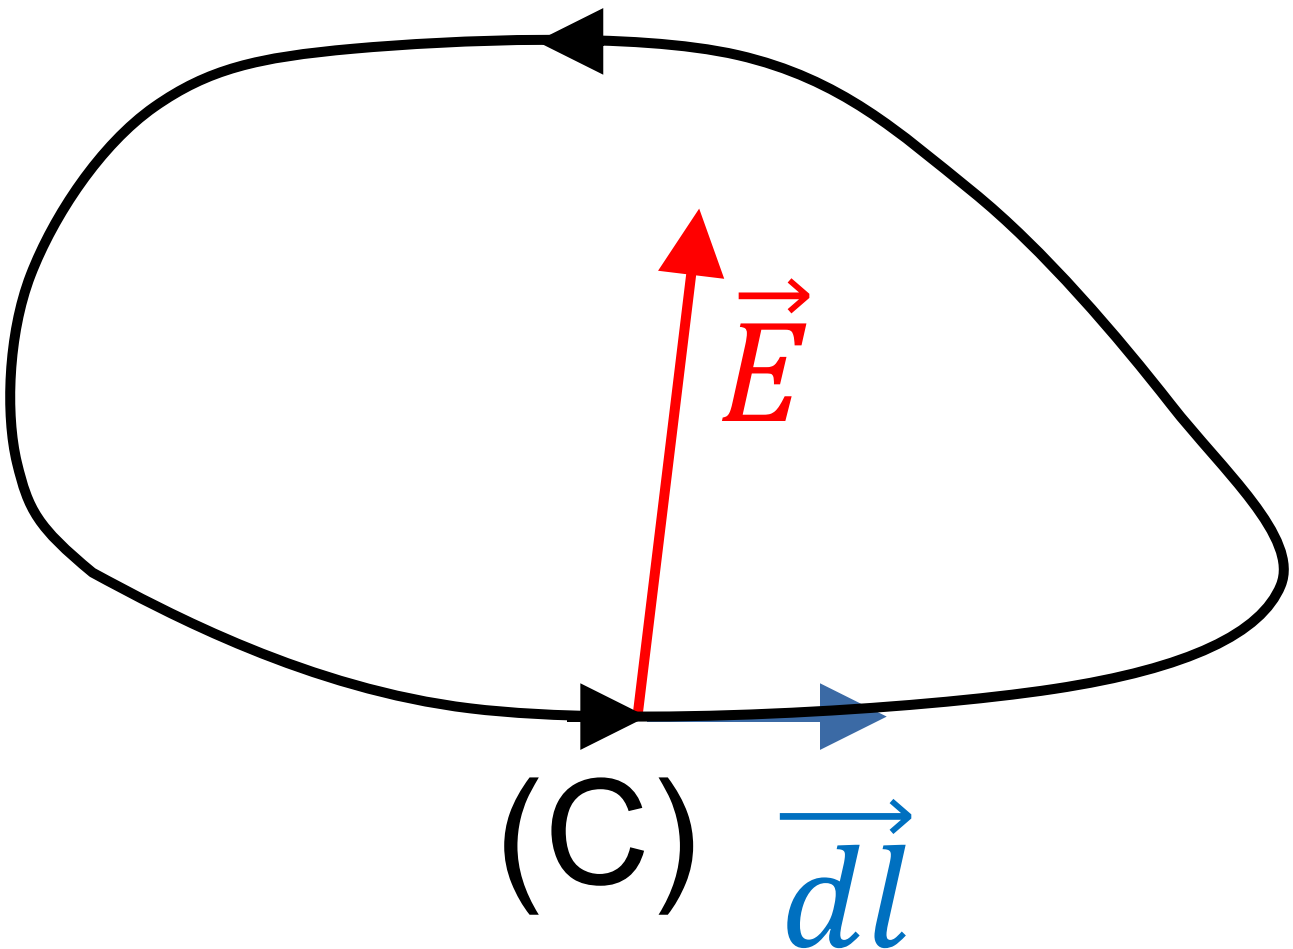
\includegraphics[width=\columnwidth]{images/V1B1.png}
\end{minipage}
\hfill
\begin{minipage}[c]{0.65\columnwidth}

    Das Kurvenintegral des elektrostatischen Feldes $\vec{E}$ 
    über jede geschlossene orientierte Kurve ($C$) ist 
    gleich null.\\
    (das elektrostatische Feld ist konservativ)

    \[
        \boxed{\underset{(A)}{\operatorname*{\oint}} \vec{E} \cdot\vec{dl} = 0}
    \]

\end{minipage}



